
% Inbuilt themes in beamer
\documentclass{beamer}
\usepackage{bbm}
\usepackage{algorithm}
\usepackage{algpseudocode}
\usepackage{tikz}
\usepackage{amsmath}
\usepackage{amssymb}
\usepackage{array}
\usepackage{graphicx}

% Theme choice:
\usetheme{Madrid}

% Title page details:
\title{Finding Diverse Strings and Longest Common Sequences in a Graph}
\subtitle{Seminar for the course of Bioinformatics}
\author{Luca Lombardo}
\date{}

\begin{document}

\begin{frame}[plain]
    \titlepage
    \begin{center}
        \footnotesize{\textit{Based on the work of: Yuto Shida, Giulia Punzi, Yasuaki Kobayashi, Takeaki Uno, Hiroki Arimura}}
    \end{center}
\end{frame}
% \logo{\large \LaTeX{}}
% \setbeamertemplate{footline}{%
%     \begin{beamercolorbox}[wd=\paperwidth,ht=2.5ex,dp=1ex,rightskip=0cm]{footline}%
%         \hspace*{1ex}%
%         \usebeamerfont{author in head/foot}\insertshortauthor\hfill%
%         \usebeamerfont{title in head/foot}\insertshorttitle%
%         \hspace*{1ex}%
%     \end{beamercolorbox}%
% }




% \begin{document}

% % Title page frame
% \begin{frame}
%     \titlepage
% \end{frame}


% Outline frame
\begin{frame}{Structure of the Presentation}
    \tableofcontents
\end{frame}

% Lists frame
\section{Introduction to the problems}
\subsection{Diverse Strings Problems}
\begin{frame}{Longest Common Subsequence (LCS)}
    \begin{definition}
        Given a set of $m$ strings $S = \{ S_1, S_2, \ldots, S_m \}$, a \textbf{common subsequence} (\emph{CS}) is a sequence that appears in all $m$ strings. A \textbf{longest common subsequence} \emph{LCS} is a common subsequence of maximum length. We denote the set of all LCSs of $S$ as $LCS(S)$.
    \end{definition}
    \begin{alertblock}{Goal}
        The goal is to find a diverse set of solutions to the LCS problem under the Hamming distance.
    \end{alertblock}
    \begin{definition}
        Given two strings $X, Y \in \Sigma^r$, the \textbf{Hamming distance} between $X$ and $Y$, denoted with $d_H(X,Y)$, is the number of positions at which the corresponding symbols differ.
    \end{definition}
\end{frame}

% \begin{frame}
%     \frametitle{A simple example}
%     % Add here the example of the paper
%     \begin{table}[h!]
%         \centering
%         \caption{Longest common subsequences of two input strings $X=ABABCDDEE$ and $Y=ABCBAEEDD.$ over $\Sigma = \{A, B, C, D, E\}$}
%         \begin{tikzpicture}
%             \node [draw, inner sep=10pt] {
%                 \begin{tabular}{>{\centering}p{10cm}}
%                     $\epsilon$, $A$, $B$, $C$, $D$, $E$,                                \\
%                     $AA$, $AB$, $AC$, $AD$, $AE$, $BA$, \ldots, $CD$, $CE$, $DD$, $EE$, \\
%                     $ABA$, $ABB$, $ABC$, $ABD$, \ldots, $CEE$,                          \\
%                     $ABAD$, $ABAE$, $ABBD$, \ldots, $BCEE$,                             \\
%                     $\underline{ABADD}$, $\underline{ABAAE}$, $\underline{ABBDD}$,      \\
%                     $\underline{ABBEE}$, $\underline{ABCDD}$, $\underline{ABCEE}$
%                 \end{tabular}
%             };
%         \end{tikzpicture}
%     \end{table}

% \end{frame}

\begin{frame}{Efficient methods for finding a diverse set of solutions}

    More formally, let's consider the following two diversity measures for a multiset $\mathcal{X} = \{X_1, X_2, \ldots, X_K\} \subseteq \Sigma^r$ of solutions, allowing repetitions:
    \begin{align}
        D_{d_H}^{\text{sum}} (\mathcal{X}) & = \sum_{1 \leq i < j \leq K} d_H(X_i, X_j) & \text{\textsc{Max-Sum Diversity}} \\
        D_{d_H}^{\text{min}} (\mathcal{X}) & = \min_{i < j} d_H(X_i, X_j)               & \text{\textsc{Max-Min Diversity}}
    \end{align}

    \begin{block}{Notation}
        A subset $\mathcal{X} \subseteq \Sigma^r$ is $\Delta$-diverse w.r.t. $D_{d_H}^{\tau}$ if $D_{d_H}^{\tau}(\mathcal{X}) \geq \Delta$ for some $\Delta \geq 0$.
    \end{block}
    Where for $\tau \in \{sum, min\}$, $D_{d_H}^{\tau}$ denotes one of the two diversity measures.
\end{frame}


\begin{frame}{Two problems}

    \begin{alertblock}{Problem 1: \textsc{Diverse LCSs with Diversity measure} $D_{d_H}^{\tau}$}
        \emph{Input:} A set $S = \{S_1, S_2, \ldots, S_m\}$ of $m \geq 2$ strings over $\Sigma$, an integer $K \geq 1$ and $\Delta \geq 0$. \\
        \emph{Question:} Is there some set $\mathcal{X} \subseteq LCS(S)$ such that $\mathcal{X}= K$ and $D_{d_H}^{\tau}(\mathcal{X}) \geq \Delta$?
    \end{alertblock}
    \begin{alertblock}{Problem 2: \textsc{Diverse String Set}}
        \emph{Input:} $K, r, \Delta \in \mathbb{Z}$ and a $\Sigma$-DAG $G$ for a set $L(G) \subseteq \Sigma^r$ of strings. \\
        \emph{Question:} Decide if there exists some subset $\mathcal{X} \subseteq L(G)$ such that $|\mathcal{X}| = K$ and $D_{d_H}^{\tau}(\mathcal{X}) \geq \Delta$.
    \end{alertblock}

\end{frame}

\subsection{$\Sigma$-DAG for LCSs}
\begin{frame}{$\Sigma$-Labeled Directed Acyclic Graphs ($\Sigma$-DAGs)}

    \begin{block}{Definitions}
        \begin{itemize}
            \item \textbf{Alphabet ($\Sigma$)}: Set of symbols.
            \item \textbf{String Set (Language)}: \( L = \{ X_1, X_2, \dots, X_n \} \subseteq \Sigma^* \), with:
                  \begin{itemize}
                      \item \textbf{Total Length}: \( ||L|| = \sum_{X \in L} |X| \)
                      \item \textbf{Max Length}: \( \text{maxLen}(L) = \max_{X \in L} |X| \)
                  \end{itemize}
            \item \textbf{r-String}: Any string \( X \) where \( |X| = r \)
        \end{itemize}
    \end{block}

    \begin{block}{$\Sigma$-DAG Structure}
        A graph \( G = (V, E, s, t) \) with:
        \begin{itemize}
            \item \( V \): vertices, \( E \): labeled edges \( (v, c, w) \) with \( c \in \Sigma \)
            \item \textbf{Source} \( s \) and \textbf{Sink} \( t \) such that paths exist from \( s \) to all vertices
            \item \textbf{Size}: \( \text{size}(G) \), the number of its labeled edges
        \end{itemize}
    \end{block}
\end{frame}


\begin{frame}{$\Sigma$-Labeled Directed Acyclic Graphs ($\Sigma$-DAGs)}
    Any path $P = (e_1, e_2, \ldots, e_n)$ of outgoing edges \emph{spells out} a string str($P$) = $c_1c_2\ldots c_n \in \Sigma^n$ where $c_i$ is the label of edge $e_i$.

    \begin{block}{Language Representation}
        A $\Sigma$-DAG represents \( L(G) \subset \Sigma^* \): all strings spelled from paths \( s \to t \). Equivalent to an NFA over $\Sigma$ with initial \( s \), final \( t \), and no $\epsilon$-edges.
    \end{block}

    \begin{exampleblock}{Remarks}
        \begin{itemize}
            \item For any set \( L \) of strings, a $\Sigma$-DAG \( G \) exists s.t. \( L(G) = L \) and \( \text{size}(G) \leq ||L|| \). Construction time: \( O(||L|| \log |\Sigma|) \).
            \item If \( G \) represents a set \( L \) of \( r \)-strings ($L \subseteq \Sigma^r, r \geq 0$), all paths \( s \to v \) have the same length $d \leq r$.
        \end{itemize}
    \end{exampleblock}

    % \begin{block}{Depth of a Vertex}
    %     \textbf{Depth} of vertex \( v \): length of path \( s \to v \). Vertices partitioned by depth.
    % \end{block}

\end{frame}

\begin{frame}{$\Sigma$-DAGs for LCSs and Diverse String Sets}

    \begin{block}{Lemma ($\Sigma$-DAG for LCSs)}
        For any constant \( m \geq 1 \) and set \( S = \{S_1, \dots, S_m\} \subseteq \Sigma^* \) of \( m \) strings, there exists a $\Sigma$-DAG \( G \) of polynomial size in \( \ell := \text{maxlen}(S) \) such that \( L(G) = \text{LCS}(S) \) and can be computed in polynomial time $l$\\
    \end{block}

    % \begin{block}{Proof (Outline)}
    %     \begin{itemize}
    %         \item Construct \( N \), an \( m \)-dimensional grid graph in \( O(\ell^m) \) time and space.
    %         \item Edge labels: Symbols from \( \Sigma \cup \{\varepsilon\} \), total edges \( O(\ell^m) \).
    %         \item \( (s, t) \)-paths in \( N \) represent LCS of \( S \).
    %         \item Apply $\epsilon$-removal to obtain a $\Sigma$-DAG \( G \) in \( O(|\Sigma| \cdot \ell^m) \) time and space.
    %     \end{itemize}
    % \end{block}

    \begin{exampleblock}{Consequence of the Lemma}
        \begin{itemize}
            \item \textbf{If} \textsc{Max-Min} (or \textsc{Max-Sum}) \textsc{Diverse String Set} solvable in \( f(M, K, r, \Delta) \),
            \item \textbf{Then} \textsc{Max-Min} (or \textsc{Max-Sum}) \textsc{Diverse LCSs} on \( S \subseteq \Sigma^r \) solvable in \( O(|\Sigma| \cdot \ell^m + f(\ell^m, K, r, \Delta)) \) time.
        \end{itemize}
        where \( \ell = \text{maxlen}(S) \)
    \end{exampleblock}

\end{frame}


\section{Exact Algorithms for Bounded Number of Diverse Strings}
% frame with just the title in the center very big
\begin{frame}
    \begin{center}
        \huge{Exact Algorithms for Bounded Number of Diverse Strings}
    \end{center}
\end{frame}


\subsection{\textsc{Max-Min Diverse String Set} problem}
\begin{frame}
    \frametitle{Algorithm for \textsc{Max-Min Diverse String Set} problem}
    % \begin{alertblock}{Brute force approach}
    %       \begin{itemize}
    %         \item \textbf{Complexity}: $O(|L(G)|^K)$ by enumerating all combinations of $K$ $(s,t)$-paths in $G$ and selecting a $\Delta$-diverse solution $\mathcal{X} \subseteq L(G)$.
    %         \item \textbf{Cons}: Impractical, $|L(G)|$ can be exponential in the number of edges
    %       \end{itemize}
    % \end{alertblock}
    \begin{block}{Dynamic Programming Approach}
        \textbf{Pattern of Path Tuple:} For each \( d \leq r \) and \( K \)-tuple of length-\( d \) paths \( P = (P_1, \dots, P_K) \),
        define pattern \( \text{Pattern}(P) = (\mathbf{w}, \mathbf{Z}) \), where:
        \begin{itemize}
            \item \( \mathbf{w} = (w_1, \ldots, w_K) \): \( K \)-tuple of vertices representing endpoints of \( P_i \) paths.
            \item \( \mathbf{Z} = (Z_{i,j}) \): Upper triangular matrix of Hamming distances, where \( Z_{i,j} = \min \{\Delta, d_H(\text{str}(P_i), \text{str}(P_j))\} \).
        \end{itemize}
    \end{block}
    \begin{block}{DP Table of Weights}
        \begin{equation}
            \text{Weights}: V^K \times (\Delta \cup \{0\})^{K \times K} \to \{0, 1\}
        \end{equation}
        Boolean matrix where \( \text{Weights}(\mathbf{w}, \mathbf{Z}) = 1 \) iff \( (\mathbf{w}, \mathbf{Z}) \) matches pattern \( \text{Pattern}(P) \) for some \( K \)-tuple of paths of length \( d \) from $s$ to $\mathbf{w}$.
    \end{block}
    % $Z$ takes at most $\Gamma = O(\Delta^{(K^2)} K^2)$ different values $\Longrightarrow$ $O(K^2 \log \Delta)$ bits
\end{frame}

\begin{frame}
    \frametitle{Algorithm for \textsc{Max-Min Diverse String Set} problem}
    % \begin{lemma}[Recurrence for Weights]
    %     $\forall ~ \mathbf{w} \in V^K$ and $\forall ~ Z = (Z_{i,j})_{i<j} \in (\Delta \cup \{0\})^{K \times K}$, the entry $\text{Weights}(\mathbf{w}, Z)$ satisfies the following:
    %     \begin{enumerate}
    %         \item \texttt{Base Case}: If $\mathbf{w} = \mathbf{s}$ and $Z = \mathbf{0}$, then $\text{Weights}(\mathbf{w}, Z) = 1$.
    %         \item \texttt{Inductive Case}: If $\mathbf{w} \neq \mathbf{s}$ and all vertices in $\mathbf{w}$ have the same depth $d$, then $\text{Weights}(\mathbf{w}, Z) = 1$ iff there exists:
    %         \begin{itemize}
    %             \item $\mathbf{v} = (v_1, \ldots, v_K) \in V_{d-1}^K$ such that each $v_i$ is a parent of $w_i$
    %             \item $U = (U_{i,j})_{i<j} \in (\Delta \cup \{0\})^{K \times K}$ such that $\text{Weights}(\mathbf{v}, U) = 1$ and $Z_{i,j} = U_{i,j} + \mathbbm{1}\{c_i \neq c_j\}$ for all $1 \leq i < j \leq K$
    %         \end{itemize}
    %         \item \texttt{Otherwise}: $\text{Weights}(\mathbf{w}, Z) = 0$.
    %     \end{enumerate}
    % \end{lemma}
    \begin{algorithm}[H] \label{alg:dp}
        \footnotesize{\caption{}}
        \footnotesize{\begin{algorithmic}[1]
                \State Set \texttt{Weights}($\mathbf{s}, Z$) $=0$ for all $Z \in (\Delta \cup \{0\})^{K \times K}$ and \texttt{Weights}($\mathbf{s}, \mathbf{0}$) $\gets 1$
                \For{$d \gets 1, \dots , r$}
                \For{$\mathbf{v} \gets (v_1, \dots v_K) \in (V_d)^K $}
                \For{$(v_1, c_1, w_1) \in E^+(v_1), \dots, (v_K, c_K, w_K) \in E^+(v_K)$}
                \State Set $\mathbf{w} = (w_1, \dots, w_K)$
                \For{$U \in (\Delta \cup \{0\})^{K \times K}$ such that \texttt{Weights}($\mathbf{v}, U$) = 1}
                \State Set $Z = (Z_{i,j})_{i<j}$ with $Z_{i,j} \gets \min \{\Delta, U_{i,j} + \mathbbm{1}\{c_i \neq c_j\}\} \quad \forall ~ i, j \in K$
                \State Set \texttt{Weights}($\mathbf{w}, Z$) $\gets 1$ \Comment{Update}
                \EndFor
                \EndFor
                \EndFor
                \EndFor
                \State Answer \texttt{Yes} if \texttt{Weights}($\mathbf{t}, Z$) = 1 and $D_{d_H}^{\text{min}}(Z) \geq \Delta$ for some $Z$, else \texttt{No}
            \end{algorithmic}}
    \end{algorithm}
    \small{For any $K \geq 1$ and $\Delta \geq 0$, it solves the \textsc{Max-Min Diverse String Set} problem in $O(\Delta^{K^2} K^2 M^K (\log |V| + \log \Delta))$ time and space when an input string set $L$ is represented by a $\Sigma$-DAG $G$ with size($G$) = $M$}
\end{frame}

% \begin{frame}
%     \frametitle{Example Run of the Algorithm}
%     \begin{figure}[h]
%         \centering
%         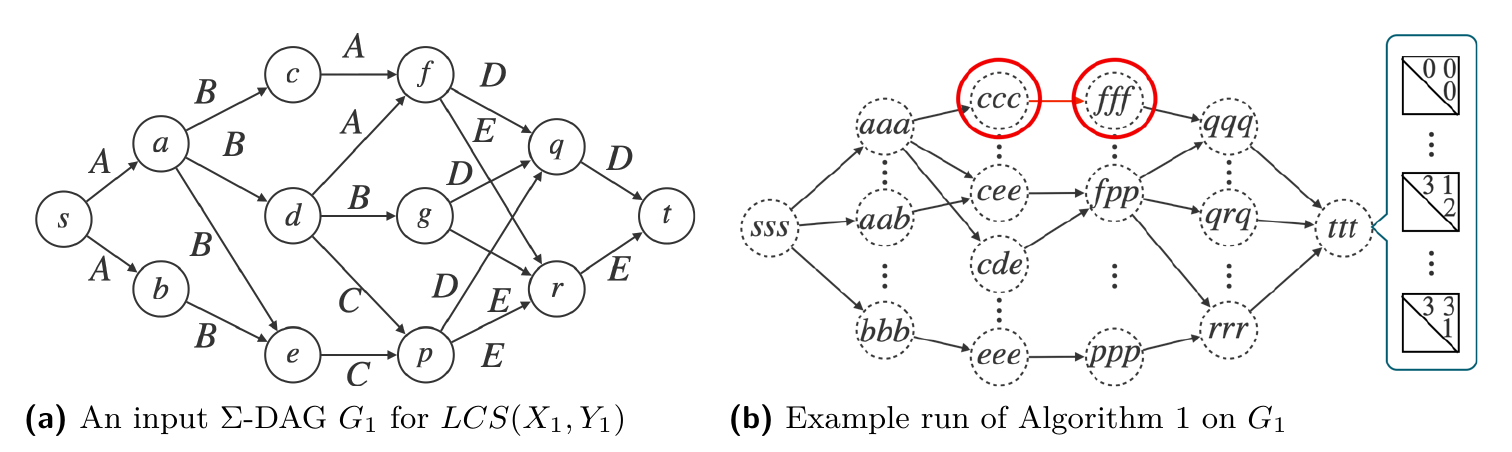
\includegraphics[width=1\textwidth]{6Kc2XEQ.png}
%         \caption{(a) An input $\Sigma$-DAG $G_1$ over $\Sigma = \{A, B, C, D, E\}$ for the set of all longest common subsequences of two strings $X_1 = \text{ABABCDDEE}$ and $Y_1 = \text{ABCBAEEDD}$ and (b) an example run of Algorithm 1 based on dynamic programming with $K = 3$ on an input $G_1$}
%         \label{fig:example}
%     \end{figure}
% \end{frame}


\subsection{\textsc{Max-Sum Diverse String Set} problem}
\begin{frame}
    \frametitle{Algorithm for \textsc{Max-Sum Diverse String Set} problem}
    \begin{block}{Modify the Max-Sum Diverse String Set problem}
        Instead of the entire \( K \times K \) weight matrix \( Z \), only the sum \( z = \sum_{i<j} d_H(\text{str}(P_i), \text{str}(P_j)) \) is needed for computing Max-Sum diversity.
    \end{block}

    \begin{block}{New DP Table Weights}
        For \( \mathbf{w} = (w_1, \dots, w_K) \) of depth \( 0 \leq d  \leq r\) and integer \( 0 \leq z \leq rK \), define:
        \[
            \texttt{Weights}(\mathbf{w}, z) = 1
        \]
        if and only if there exists a \( K \)-tuple of length-\( d \) prefix paths \( (P_1, \dots, P_K) \) from \( s \) to \( w_1, \dots, w_K \) with sum of pairwise Hamming distances \( z \).
    \end{block}

\end{frame}

\begin{frame}
    \frametitle{Algorithm for \textsc{Max-Sum Diverse String Set} problem}
    \begin{algorithm}[H] \label{alg:dp2}
        \footnotesize{\caption{}}
        \footnotesize{\begin{algorithmic}[1]
                \State Set \texttt{Weights}($\mathbf{s}, Z$) $=0$ for all $Z \in (\Delta \cup \{0\})^{K \times K}$ and \texttt{Weights}($\mathbf{s}, \mathbf{0}$) $\gets 1$
                \For{$d \gets 1, \dots , r$}
                \For{$\mathbf{v} \gets (v_1, \dots v_K) \in (V_d)^K $}
                \For{$(v_1, c_1, w_1) \in E^+(v_1), \dots, (v_K, c_K, w_K) \in E^+(v_K)$}
                \State Set $\mathbf{w} = (w_1, \dots, w_K)$
                \For{$u \gets (0, \dots, rK)$ such that \texttt{Weights}($\mathbf{v}, U$) = 1}
                \State Set $Z = (Z_{i,j})_{i<j}$ with $Z_{i,j} \gets \min \{\Delta, u + \sum_{i<j}\mathbbm{1}\{c_i \neq c_j\}\}$
                \State Set \texttt{Weights}($\mathbf{w}, Z$) $\gets 1$ \Comment{Update}
                \EndFor
                \EndFor
                \EndFor
                \EndFor
                \State Answer \texttt{Yes} if \texttt{Weights}($\mathbf{t}, Z$) = 1 and $D_{d_H}^{\text{min}}(Z) \geq \Delta$ for some $Z$, else \texttt{No}
            \end{algorithmic}}
    \end{algorithm}
    \small{For any $K \geq 1$, it solves the \textsc{Max-Sum Diverse String Set} under Hamming Distance in $O(\Delta K^2 M^K (\log |V| + \log \Delta))$ time and space, where $M$ is the size of the input $\Sigma$-DAG $G$}
\end{frame}

\section{Approximation Algorithms for Unbounded Number of Diverse Strings}
\begin{frame}
    \begin{center}
        \huge{Approximation Algorithms for Unbounded Number of Diverse Strings}
    \end{center}
\end{frame}

\subsection{Approximation Algorithm for \textsc{Max-Min Diverse String Set} problem}
\begin{frame}
    \frametitle{\textsc{Max-Sum Diverse String Set} problem}
    Use a local search algorithm for computing approximate solutions $\mathcal{X} \subseteq \mathcal{L}$ with $|\mathcal{X}| = K$ on a finite metric space $(\mathcal{L}, d)$, where $d: \mathcal{L} \times \mathcal{L} \to \mathbb{R}_{\geq 0}$.

    \begin{algorithm}[H] \label{alg:LocalSearch}
        \footnotesize{\caption{\texttt{LocalSearch}($\mathcal{L}, K, d$)}}
        \footnotesize{\begin{algorithmic}[1]
                \State $\mathcal{X} \gets$ arbitrary set of $K$ solutions in $\mathcal{L}$
                \For{$i \gets 1, \dots, \lceil \frac{K(K-1)}{K+1} \log \frac{(K+2)(K-1)^2}{4} \rceil$}
                \For{$X \in \mathcal{X}$ s.t $\mathcal{L} \setminus \{X\} \neq \emptyset$}
                \State $Y \gets \text{argmax}_{Y \in \mathcal{L} \setminus \{X\}} \sum_{X' \in \mathcal{X} \setminus \{X\}} d(X', Y)$
                \State $\mathcal{X} \gets \mathcal{X} \setminus \{X\} \cup \{Y\}$
                \EndFor
                \EndFor
                \State \textbf{return} $\mathcal{X}$
            \end{algorithmic}}
    \end{algorithm}

    \begin{theorem}
        \small{When the distance $d$ is a semi-metric of \emph{negative type} over $\mathcal{X}$, then \textsc{LocalSearch} has improved approximation ratio $(1 - \frac{2}{K})$ for any $K \geq 2$. The Hamming distance $d_H$ over the set of $r$-strings is a semi-metric of negative type.}
    \end{theorem}
\end{frame}

\begin{frame}
    \frametitle{\textsc{Max Sum Farthest} r-\textsc{String} problem}
    How do we solve efficiently the following problem?
    \[
        Y \gets \text{argmax}_{Y \in \mathcal{L} \setminus \{X\}} \sum_{X' \in \mathcal{X} \setminus \{X\}} d(X', Y)
    \]
    % The following algorithm can be modified to compute such $Y$ by reordering the parent pair $(v, y)$ of each $(w, z)$ and then tracking back
    % start an algorithm environment
    \begin{algorithm}[H] \label{alg:ExactMaxSumFarthest}
        \small{\caption{Decisional \textsc{Max-Sum Farthest} r-\textsc{String}}}
        \footnotesize{\begin{algorithmic}[1]
                \State Set $Weights(s, z) := 0$ for all $z \in [\Delta]_+$, and $Weights(s, 0) := 1$\;
                \For{$d := 1, \dots, r$}
                \For{$0\le u\le \Delta$ such that $Weights(v, u) := 1$}
                \State Set $Weights(w, z) := 1$ for $z := u + \sum_{i \in [K]} \mathbbm{1}\{ c \not= X_i[d] \}$ \Comment{Update}
                \EndFor
                \EndFor
                \State Answer YES if $Weights(t, \Delta) = 1$, and NO otherwise \Comment{Decide}
            \end{algorithmic}}
    \end{algorithm}
    \begin{theorem}[Polynomial Time Approximation Scheme for unbounded $K$]
        When $K$ is part of an input, \textsc{Max-Sum Diverse String Set} problem on a $\Sigma$-DAG admits a PTAS
    \end{theorem}
\end{frame}

% \begin{frame}
%     \frametitle{\textsc{Max-Sum Farthest} r-\textsc{String} problem}

%     \begin{lemma}[Max-Sum Farthest $r$-String]
%         For any $K \geq 1$ and $\Delta \geq 0$, \textsc{Algorithm 3} computes the farthest $r$-string $Y \in L(G)$ that maximizes $D_{d_H}^{\text{sum}}(Y \cup \mathcal{X})$ over all $r$-strings in $L(G)$ in $O(K \Delta M)$ time and space, where $M$ is the size of the input $\Sigma$-DAG $G$.
%     \end{lemma}

%     \begin{theorem}[Polynomial Time Approximation Scheme for unbounded $K$]
%         When $K$ i part of an input, \textsc{Max-Sum Diverse String Set} problem on a $\Sigma$-DAG admits a PTAS
%     \end{theorem}
%     The corresponding result for the \textsc{Max-Sum Diverse LCSs} follows immediately.

% \end{frame}

\section{FPT Algorithms for Bounded Number and Length of Diverse Strings}
\begin{frame}
    \begin{center}
        \huge{Fixed-Parameter Tractable (FPT) Algorithms for Bounded Number and Length of Diverse Strings}
    \end{center}
\end{frame}

\begin{frame}
    \frametitle{FPT Algorithms for \textsc{Max-Min} and \textsc{Max-Sum Diverse String Set} problems}
    \begin{definition}[Fixed-Parameter Tractable (FPT) Algorithm]
        A problem parametrized with $\kappa$ is said to be \emph{fixed-parameter tractable} (FPT) if there exists an algorithm for the problem running on an input $x$ in time $f(\kappa (x) \cdot |x|^c)$, where $f$ is a computable function and $c > 0$ is a constant.
    \end{definition}
    \begin{block}{Proposed FPT Algorithm}
        \textit{Color-coding} technique with dynamic programming to solve these problems efficiently. Assign a random color to the edges of the $\Sigma$-DAG $G$, creating a colored graph called $C$-DAG, then reduce it to a trie $T$.
    \end{block}
    \begin{theorem}
        For any set $C$ of $k$ colors, there exists some $C$-DAG $H$ obtained by reducing $c(G)$ such that $L(H) = L(c(G))$ and $||H|| \le k^r$.
    \end{theorem}
    % \begin{theorem}
    %     When $r, K, \Delta$ are part of the input, the \textsc{Max-Min Diverse String Set} problem on a $\Sigma$-DAG admits an FPT algorithm.
    % \end{theorem}
    % \begin{theorem}
    %     When $r, K, \Delta$ are part of the input, the \textsc{Max-Sum Diverse String Set} problem on a $\Sigma$-graphs for $r$-strings admits an FPT algorithm.
    % \end{theorem}

\end{frame}

\begin{frame}
    \frametitle{Computation of Reduced $C$-DAG}
    \begin{figure}[t]
        \abovecaptionskip=-0.0\baselineskip
        %\belowcaptionskip=-0.5\baselineskip
        \centering
        \vspace{-0.5\baselineskip}
        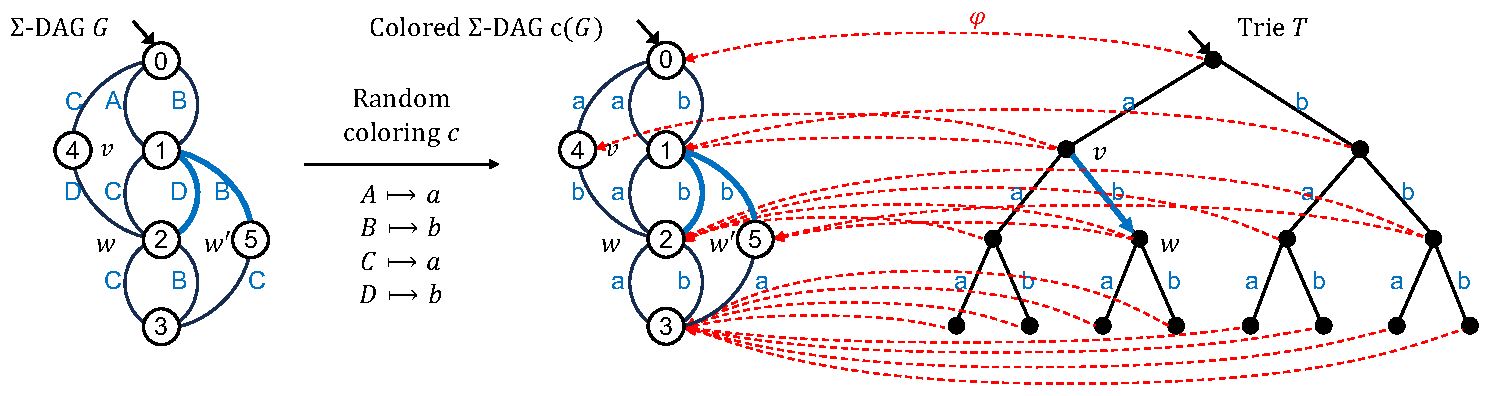
\includegraphics[width=0.9\textwidth,angle=0]{./figfptalgo}
        \caption{Computation of reduced $C$-DAG $H$ from an input $\Sigma$-DAG $G$ over alphabet $\Sigma = \{A, B, C, D\}$ , which shows $G$  (left), a random coloring $c$ on $C = \{a,b\}$, a colored $C$-DAG $c(G)$ (middle), and a reduced $C$-DAG $H$ in the form of trie $T$ (right)}\label{fig:fptalgo}
    \end{figure}

    % \begin{theorem}{}
    %     An analogous FPT algorithm can be designed for the \textsc{Max-Sum Diverse String Set} problem with a small modification in the research phase, that, in this case, is  $O(\Delta K^2 M^K)$
    % \end{theorem}
    \begin{theorem}{}
        When $r$ and $K$ are parameters, the \textsc{Max-Min (Max-Sum) Diverse String Set}
        on a $\Sigma$-DAG for $r$-strings is fixed-parameter tractable (FPT), where $size(G)$ is
        an input.
    \end{theorem}

\end{frame}

\section{Complexity Results for Diverse String Problems}

\begin{frame}{Complexity Results for Diverse String Problems}
    \begin{block}{Negative Results}
        \begin{itemize}
            \item NP-hard for unbounded $K$ (\textsc{Max-Min}, \textsc{Max-Sum}) in $\Sigma$-graphs for $r$-strings, $r \ge 3$.
            \item W[1]-hard parameterized with $K$ for $\textsc{Max-Min}$ and $\textsc{Max-Sum}$ in $\Sigma$-DAGs.
        \end{itemize}
    \end{block}

    \begin{block}{Reduction to Diverse LCSs}
        \textsc{Max-Min} and \textsc{Max-Sum} problems are FPT-reducible to \textsc{Diverse LCSs} for $m=2$ strings.
    \end{block}

    \begin{block}{Corollaries}
        NP-hard and W[1]-hard results extend to \textsc{Diverse LCSs} for two $r$-strings.
    \end{block}
\end{frame}

\section*{Conclusions}
\begin{frame}
    \frametitle{Conclusion}

    \begin{itemize}
        \item \textbf{Polynomial-Time Solutions}: When \( K \) is bounded, both the \textsc{Max-Sum} and \textsc{Max-Min} versions of \textsc{Diverse String Set} and \textsc{Diverse LCSs} can be solved in polynomial time using dynamic programming (DP).
        \item \textbf{PTAS for Input-Based \( K \)}: For input-dependent \( K \), the \textsc{Max-Sum} versions of both \textsc{Diverse String Set} and \textsc{Diverse LCSs} admit a PTAS using local search due to the Hamming distance being a metric of negative type.
        \item \textbf{Fixed-Parameter Tractability (FPT)}: Both versions are FPT when parameterized by \( K \) and \( r \), combining the color coding technique and DP.
        \item \textbf{NP-Hardness for Constant \( r \ge 3 \)}: When \( K \) is part of the input, both the \textsc{Max-Sum} and \textsc{Max-Min} versions are NP-hard for any constant \( r \ge 3 \).
        \item \textbf{W[1]-Hard for Parameterized \( K \)}: Parameterized by \( K \), both versions are W[1]-hard.
    \end{itemize}

\end{frame}



% \section{Hardness Results}
% \subsection{Hardness of Diverse String Set for Unbounded $K$}

% \begin{frame}
%     \frametitle{Hardness results}
%     \begin{theorem}[NP-Hardness for unbounded $K$]
%         When $K$ is part of the input, the \textsc{Max-Min Diverse String Set} and \textsc{Max-Sum Diverse String Set} problems on a $\Sigma$-graph for $r$-strings are NP-hard even for any constant $r \geq 3$.
%     \end{theorem}
%     \begin{theorem}[Hardness of Diverse LCSs for Unbounded $K$]
%         Under Hamming distance, the \textsc{Max-Min} (resp. \textsc{Max-Sum}) \textsc{Diverse Set} for $m \geq 2$ strings
%     \end{theorem}
% \end{frame}

% \subsection{Hardness of Diverse String LCSs for Unbounded $K$}
% \begin{frame}
%     \frametitle{Hardness of Diverse String LCSs for Unbounded $K$}

% \end{frame}


\end{document}
